
\chapter{Debayer}
As the polarization images taken by the \cams use a custom raw format, no existing software can be used to process the images efficiently.
One of the major contributions of the thesis is the implementation of an optima

\subsection{Debayering}
Debayering is the process of estimating complete color information for an image that has been captured through a \gls{cfa}, particularly on the Bayer pattern \cite{getreuerMalvarHeCutlerLinearImage2011}.
In the Bayer pattern, green pixels cover half the array in a lattice, and the red and blue pixel locations are spaced uniformly every two pixels shown in figure \ref{fig:debayer:bayer_pattern} \cite{getreuerMalvarHeCutlerLinearImage2011}.
Different orderings of the colors exists, with the most common ones being RGGB, BGGR, GRBG, and GBRG, but the concepts stays the same.

Debayering involves interpolating the missing color information from the \gls{cfa} data.
Malvar, He, and Cutler proposed a simple linear method using 5 x 5 filters that shows surprisingly good results \cite{getreuerMalvarHeCutlerLinearImage2011}.
The method they present is derived as a modification of bilinear interpolation, and it involves adding Laplacian cross-channel corrections to improve the quality of the bilinear method.
The demosaicking is implemented by convolution with a set of linear filters, and there are eight different filters for interpolating the different color components at different locations as can be shown in figure \ref{fig:debayer:malvar_filters}.
The method is more suited for parallel execution than many others as discussed in \todo.


\begin{figure}[tb]
    \centering
    \begin{tabular}[b]{ccc}
        \subcaptionbox{RGGB bayer pattern}{
            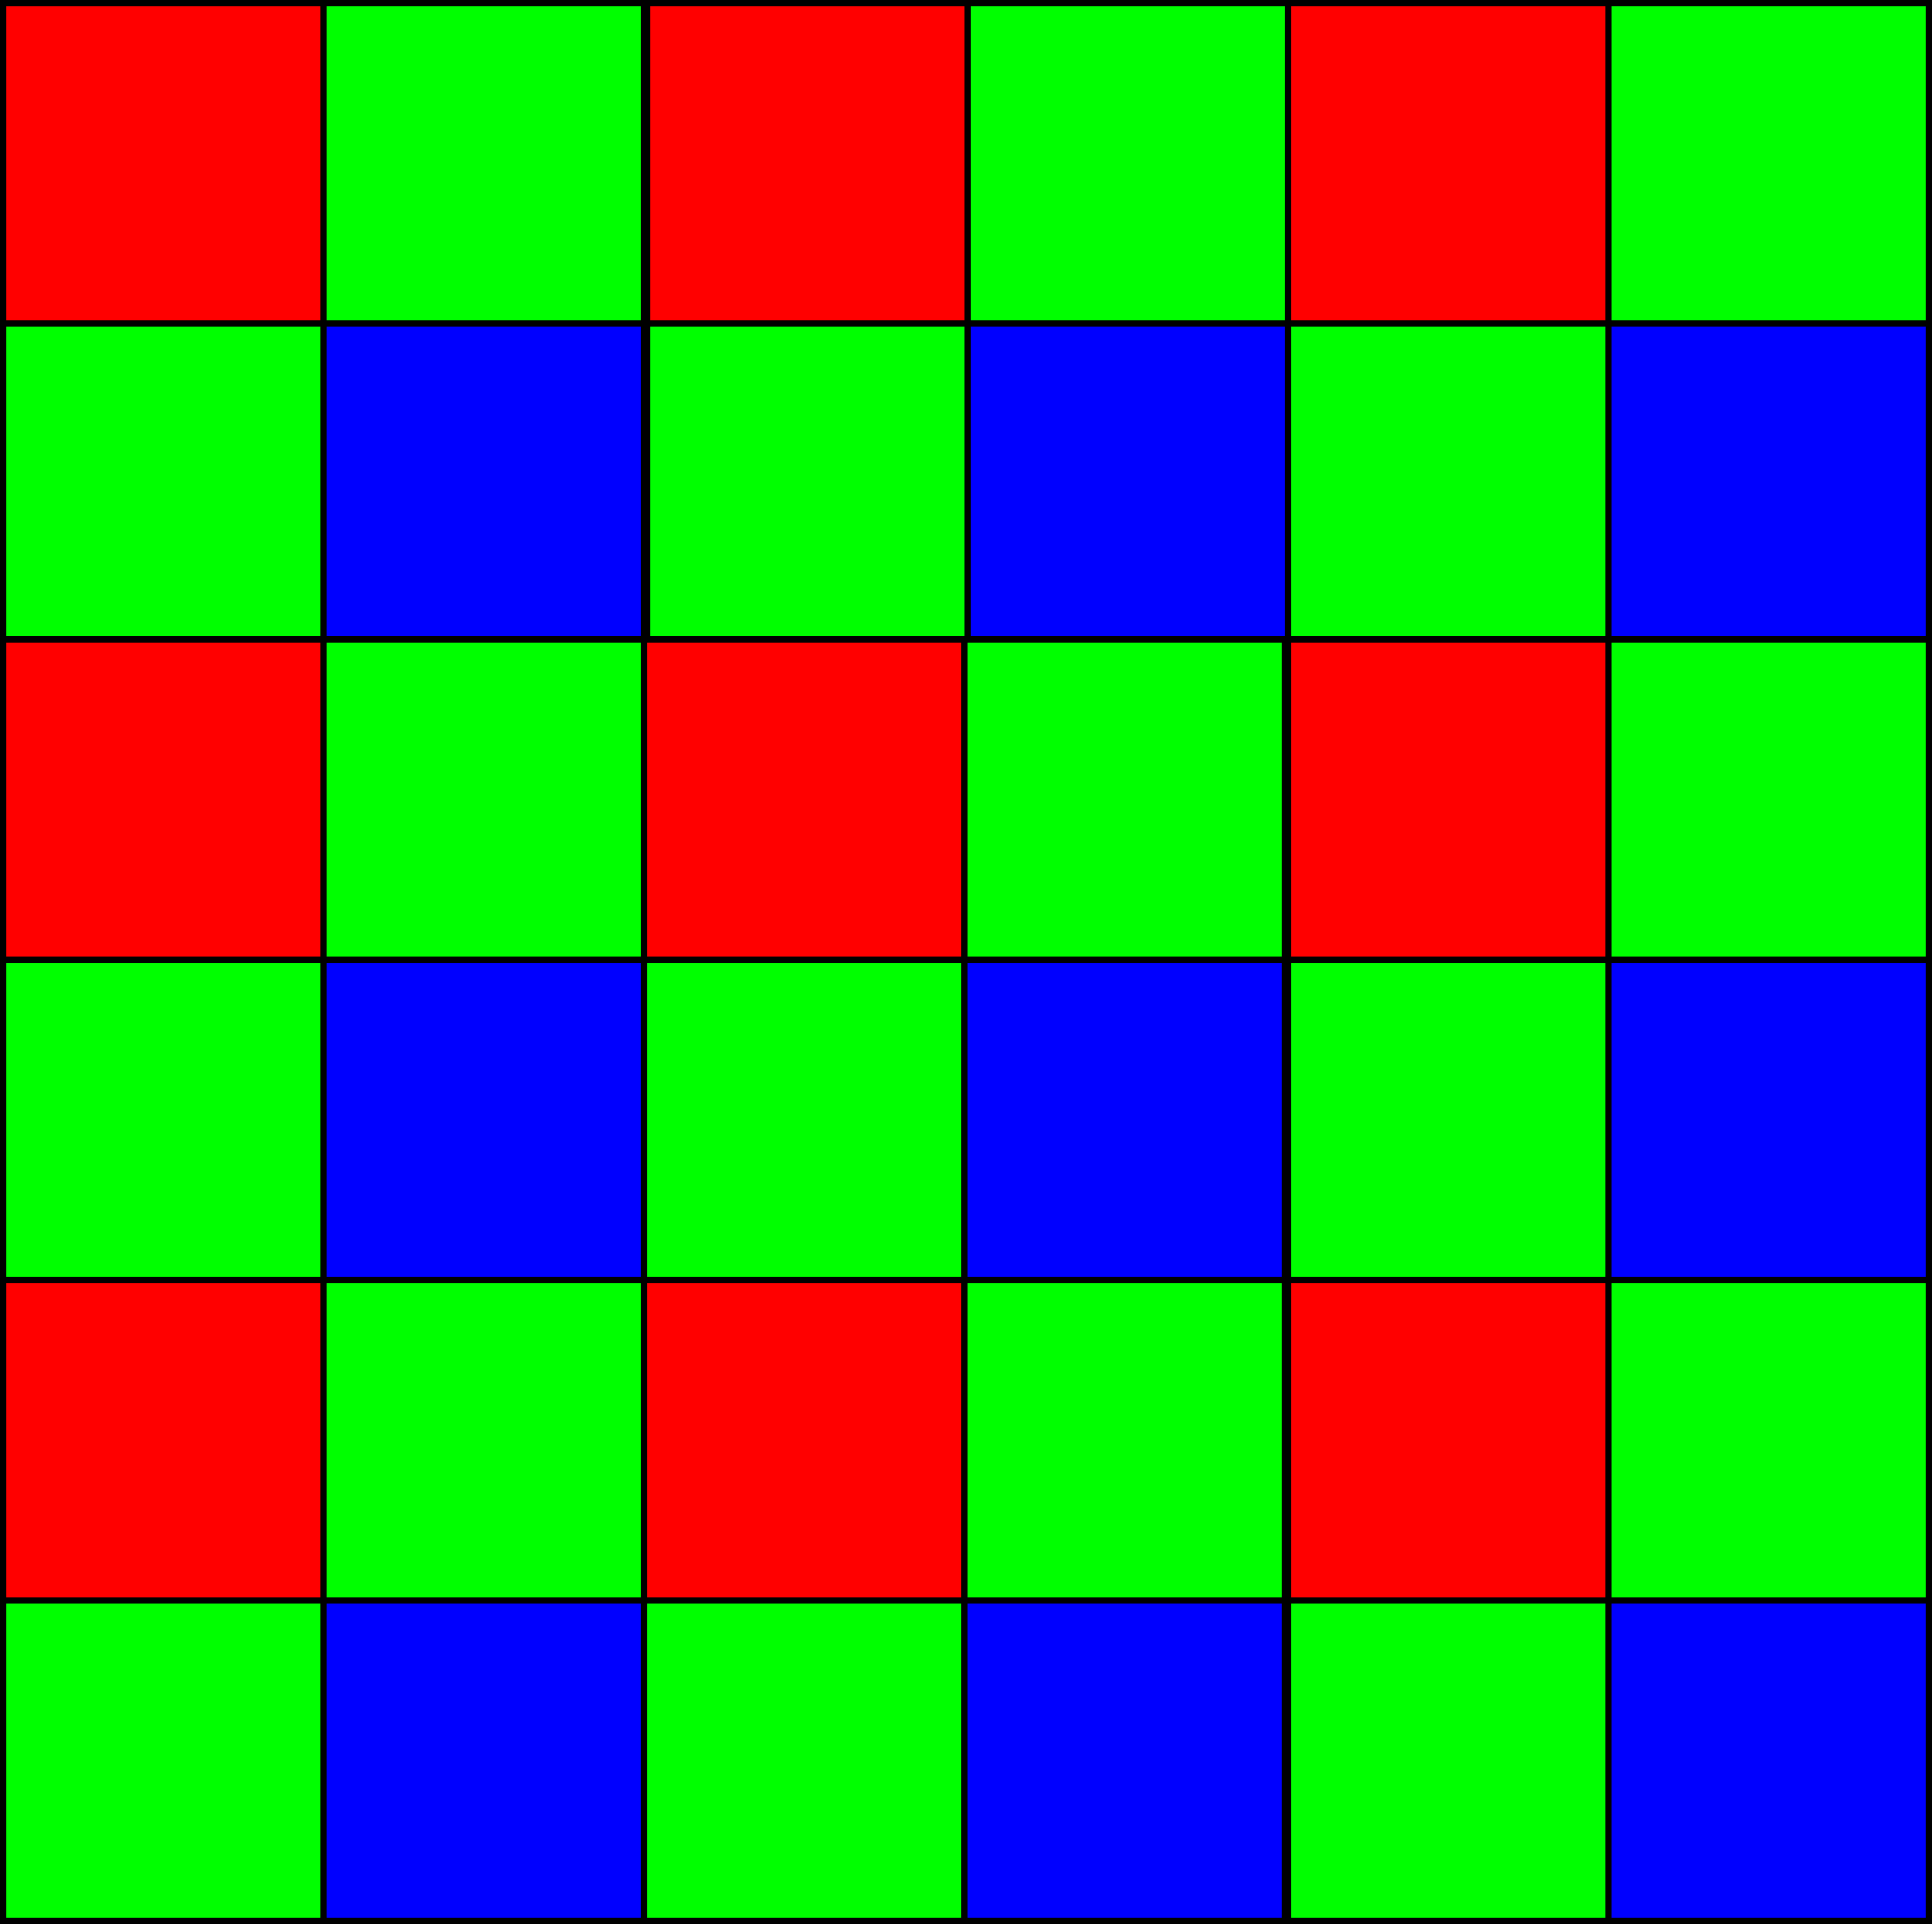
\includegraphics[width=0.25\textwidth]{figures/debayer/bayer_pattern.pdf}
            \label{fig:debayer:bayer_pattern}
        } &
        \subcaptionbox{Green at red}{
            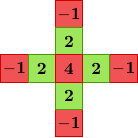
\includegraphics[width=0.25\textwidth]{figures/debayer/g_at_r.png}
        } &
        \subcaptionbox{Green at red}{
            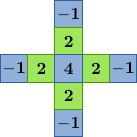
\includegraphics[width=0.25\textwidth]{figures/debayer/g_at_b.png}
        }
        \\
        \subcaptionbox{Red at }{
            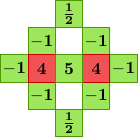
\includegraphics[width=0.25\textwidth]{figures/debayer/r_at_g_rr.png}
        } &
        \subcaptionbox{Red at green, blue row}{
            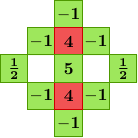
\includegraphics[width=0.25\textwidth]{figures/debayer/r_at_g_br.png}
        } &
        \subcaptionbox{Red at blue}{
            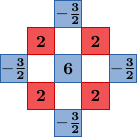
\includegraphics[width=0.25\textwidth]{figures/debayer/r_at_b.png}
        }
        \\
        \subcaptionbox{Blue at green, red row}{
            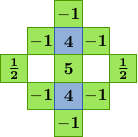
\includegraphics[width=0.25\textwidth]{figures/debayer/b_at_g_rr.png}
        } &
        \subcaptionbox{Blue at green, blue row}{
            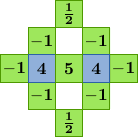
\includegraphics[width=0.25\textwidth]{figures/debayer/b_at_g_br.png}
        } &
        \subcaptionbox{Blue at red}{
            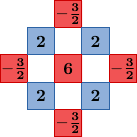
\includegraphics[width=0.25\textwidth]{figures/debayer/b_at_r.png}
        }
    \end{tabular}
    \caption{Coefficient values used by Malvar-He-Cutler scaled by 8 \cite{getreuerMalvarHeCutlerLinearImage2011}\cite{CommonsBayerPattern2020}}
    \label{fig:debayer:malvar_filters}
\end{figure}

\begin{figure}[tb]
    \centering
    \begin{tabular}[b]{ccc}
        \subcaptionbox{Exact image}{
            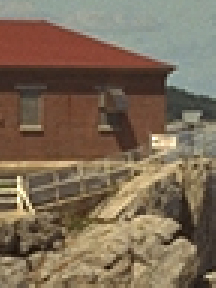
\includegraphics[width=0.3\textwidth]{figures/debayer/house_orig.jpg}

        } &
        \subcaptionbox{Observed Image}{
            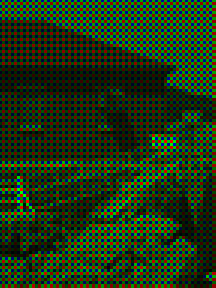
\includegraphics[width=0.3\textwidth]{figures/debayer/house_bayer.png}
        }
        \\
        \subcaptionbox{Bilinear (PSNR=25.61)}{
            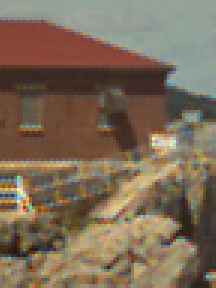
\includegraphics[width=0.3\textwidth]{figures/debayer/house_bilinear.png}
        } &

        \subcaptionbox{Hamilton-Adams \todo (PSNR=31.62)}{
            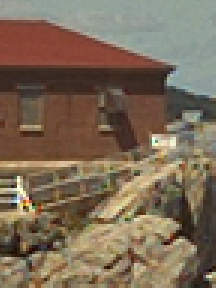
\includegraphics[width=0.3\textwidth]{figures/debayer/house_hamilton.png}
        } &
        \subcaptionbox{Malvar-He-Cutler (PSNR=31.15)}{
            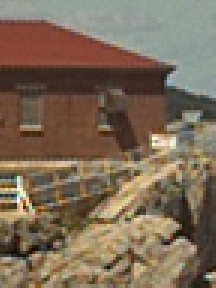
\includegraphics[width=0.3\textwidth]{figures/debayer/house_malvar.png}
        }
    \end{tabular}
    \caption{Coefficient values used by Malvar-He-Cutler scaled by 8 \cite{getreuerMalvarHeCutlerLinearImage2011}}
\end{figure}
\section{GPU programming in CUDA}
In recent years, there has been a significant shift towards parallel computing in order to achieve faster processing times and better performance.
The rise of \glspl{gpu} has been a major factor in enabling parallel computing for a wide range of applications, from machine learning to scientific simulations.
One of the most popular platforms for parallel computing on GPUs is \gls{cuda} developed by NVIDIA, which is a framework and programming model for parallel computing on NVIDIA \glspl{gpu}.

CUDA is a parallel computing platform and programming model developed by NVIDIA that allows developers to harness the power of their GPUs for a wide range of applications.

Programming for GPUs is fundamentally different from programming for CPUs.
While CPUs have a small number of powerful cores, GPUs have a much larger number of simpler cores.
This means that code needs to be structured differently to take advantage of the parallelism offered by GPUs.
In addition, data transfer between the CPU and GPU can be a bottleneck, so care must be taken to optimize data movement.

In this chapter, we will explore the basics of CUDA programming, including the key differences between programming for CPUs and GPUs, and the general workflow of programming in CUDA.
We will cover topics such as device memory management, kernel functions, and thread synchronization.


\subsection{Heterogeneous Computing}
Heterogeneous computing refers to a programming model where multiple different types of computing cores cooporate to solve groups of tasks in an efficient manner \cite{armWhatHeterogenousCompute}.
The \jx is a good example of this; equiped with an 8-core ARM \gls{cpu} and a 512-core NVIDIA \gls{gpu}, as well as an \gls{isp}, \gls{dla} and two \glspl{nvenc} for specific media encoding and decoding tasks among other thing \cite[9, 8, 23, 15-22]{nvidiaNVIDIAJetsonAGX2019}.
This combination of different types of cores working together allows for a system to efficiently handle a wide range of tasks, from general-purpose computing to specialized tasks such as video processing and compression.

\begin{figure}
    \centering
    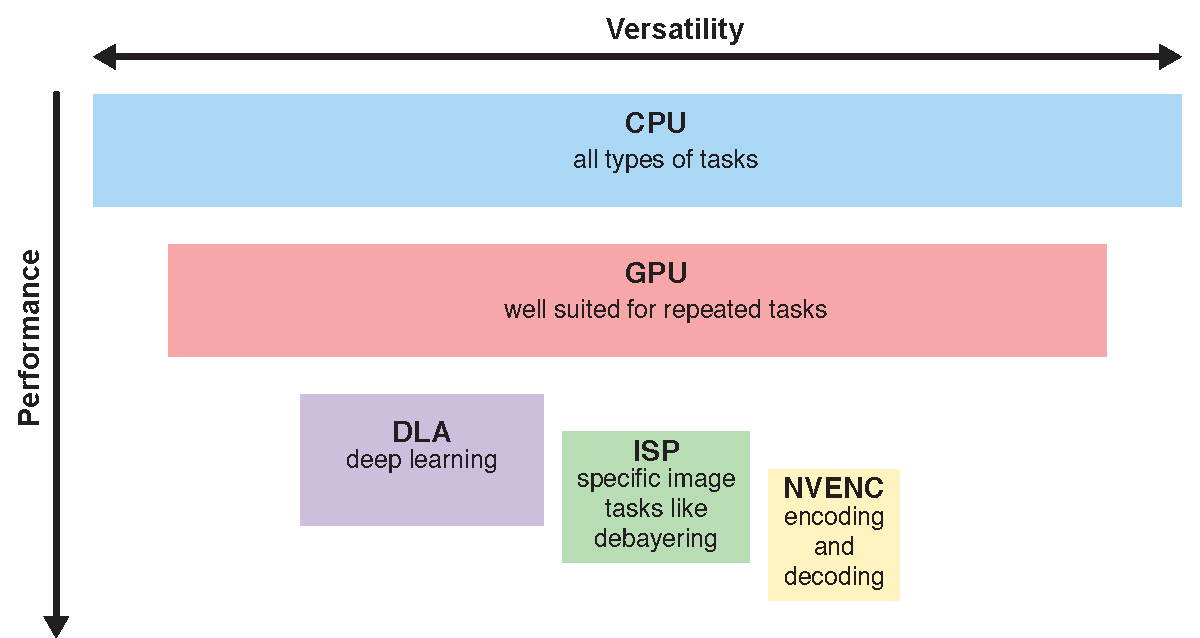
\includegraphics[width=\textwidth]{figures/PDF/jx_hierarchy.pdf}
    \caption{Illustration of the versatility and performance of different types of cores on the \jx.}
    \label{fig:jx_hierarchy}
\end{figure}


\subsubsection{Memory Management}
With different types of cores comes different types of memory.
A key challenge of working with heterogeneous computing systems is to manage the different types of memory efficiently, so that the different cores have access to the data they need when they need it.

A major advantage of working on the \jx is the posibility to share memory between the different types of cores, removing the need for expensive data transfers between the different types of memory.
This is further discussed in Section \ref{sec:jx_memory}.

\begin{figure}
    \centering
    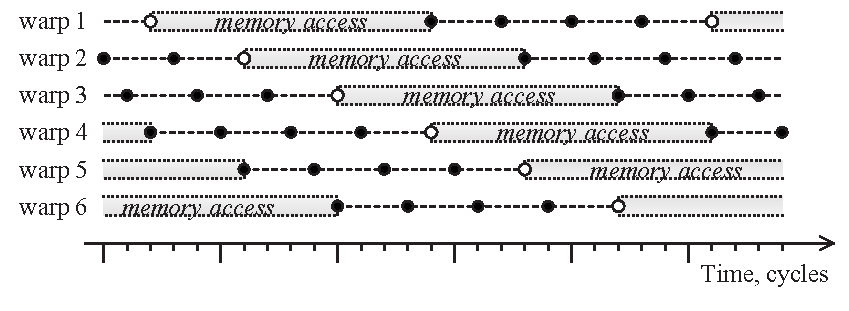
\includegraphics[width=\textwidth]{figures/PDF/concurrency_p54.pdf}
    \caption{Visualization of concurrent execution on a GPU \cite[54]{VolkovLatencyHiding2016}}
    \label{fig:concurrency}
\end{figure}


\subsubsection{Latency Hiding}
Latency hiding is a technique used by modern commodity processors such as GPUs to better utilize their numerous execution units and hide execution latencies \cite[35]{Volkov:EECS-2016-143}
The idea behind latency hiding is to keep the processor busy with other tasks while it waits for data to be fetched from memory.
This is achieved by executing multiple threads in parallel, so that when one thread is waiting for data, another thread can continue executing.


\subsubsection{Profiling}
Profiling is the process of measuring the performance of a program, and is an important tool for optimizing programs.

In many cases it is straight forward; record the time when a task is started and when it is finished, and calculate the difference.


However, when working with heterogeneous computing systems, it is not always


\subsection{Heterogeneous}
\subsection{Heterogeneous}
\subsection{Heterogeneous}
\subsection{Heterogeneous}
\subsection{Unpacking}
The \lucid cameras are capable of
\begin{figure}
    \centering
    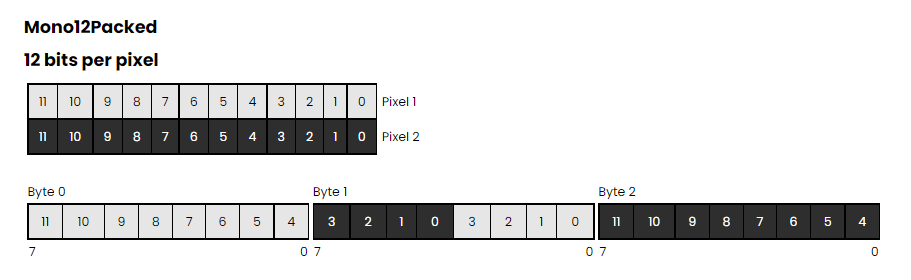
\includegraphics[width=\textwidth]{figures/Mono12Packed.png}
    \caption{Bit layout of the \cite{fisherRe15406LUT2023}}
    \label{fig:mono12packed}
\end{figure}

\begin{listing}[H]
    \begin{minted}{cuda}
        template <int width, int width_in>
        __device__ __forceinline__ void unpack10(__half2 *work_row, 
                                                 const unsigned int *img_row,
                                                 int tx) {
            __half2 *const out = &work_row[tx * 8 + 2];
        
            if (tx * 5 < width_in) {
                unsigned int buf_a, buf_b;
                buf_a = img_row[tx * 5];
                buf_b = img_row[tx * 5 + 1];
                out[0] = __halves2half2(buf_a & 0b1111111111, 
                                        buf_a >> 10 & 0b1111111111);
                out[1] = __halves2half2(buf_a >> 20 & 0b1111111111,
                                        buf_a >> 30 & 0b11 | (buf_b & 0b11111111) << 2);
        
                buf_a = img_row[tx * 5 + 2];
                out[2] = __halves2half2(buf_b >> 8 & 0b1111111111, 
                                        buf_b >> 18 & 0b1111111111);
                out[3] = __halves2half2(buf_b >> 28 & 0b1111 | (buf_a & 0b111111) << 4,
                                        buf_a >> 6 & 0b1111111111);

                buf_b = img_row[tx * 5 + 3];
                out[4] = __halves2half2(buf_a >> 16 & 0b1111111111,
                                        buf_a >> 26 & 0b111111 | (buf_b & 0b1111) << 6);
                out[5] = __halves2half2(buf_b >> 4 & 0b1111111111, 
                                        buf_b >> 14 & 0b1111111111);
        
                buf_a = img_row[tx * 5 + 4];
                out[6] = __halves2half2(buf_b >> 24 & 0b11111111 | (buf_a & 0b11) << 8,
                                        buf_a >> 2 & 0b1111111111);
                out[7] = __halves2half2(buf_a >> 12 & 0b1111111111, 
                                        buf_a >> 22 & 0b1111111111);
            }
            if (tx < 2) {
                work_row[tx] = work_row[tx + 2];
            } else if (tx >= width - 2 && tx < width) {
                work_row[tx + 4] = work_row[tx + 2];
            }
        }
    \end{minted}
    \caption{Bit unpacking in \cuda}
\end{listing}
\section{Memory management on Jetson platform}
\label{sec:jx_memory}
On \gls{tegra} platforms, there are different types of memory available for use, including device memory, pageable host memory, pinned memory, and unified memory docs.nvidia.com.
These memory types are allocated on the same physical SoC DRAM but have different accessing and caching behaviors.
Device memory is used for buffers limited to \gls{igpu} access, pageable host memory is used for buffers limited to CPU access, pinned memory is recommended for small buffers, and unified memory is cached on both \gls{igpu} and CPU \cite{nvidiaCUDAFTegra2023}.


\subsection{Memory types}
This section presents the different memoty types available on the \jx.
It builds upon the CUDA for Tegra documentation \cite{nvidiaCUDAFTegra2023}, with a focus on what is relevant for the setup on the \sr, where ther is a \jx with compute cabability of 7.2 \cite{CUDA2023} and no external \gls{dgpu}.
A summary of the different memory types is presented in Table \ref{tab:memory_types}.


\providecommand{\tmpfootnote}{\footnote{Cached where compute capability is greater than or equal to 7.2 \cite
        {nvidiaCUDAFTegra2023}. The \jx has compute capability of 7.2 \cite{CUDA2023} }}
\begin{table}
    \centering
    \begin{tabular}{ |c|c|c| }
        \hline
        \textbf{Memory Type} & \textbf{CPU}            & \textbf{iGPU}           \\
        \hline
        Pageable host memory & Cached                  & Not directly accessible \\
        Device memory        & Not directly accessible & Cached                  \\
        Pinned host memory   & Cached                  & Uncached                \\
        Pageable host memory & Cached                  & Cached                  \\
        \hline
    \end{tabular}
    \caption{Memory types on the \jx \cite{nvidiaCUDAFTegra2023}}
    \label{tab:memory_types}
\end{table}
\subsubsection{Pageable host memory}
Pageable host memory, is the normal type of memory used on the \jx,
e.g. it is what is used allocated with \code{malloc} and used to store normal \py objects.
When memory is pageable the \cpu can control where it is stored, and it can be moved to the \gls{swap} area to free up physical memory \cite[6]{nvidiaCUDAFTegra2023}.
This is why it is not directly accessible by the \gls{igpu}.
If memory is not accesed by the \gls{igpu}, pageable memory should be used \cite[9]{nvidiaCUDAFTegra2023}


\subsubsection{Device memory}
Device memory is memory that is directly accessible by the \gls{igpu} but not the \cpu \cite[5]{nvidiaCUDAFTegra2023}.
It is allocated on the same physical SoC DRAM as other memory types, but cached in a way that is optimized for \gpu usage, making in unacessable on the \cpu \cite[5]{nvidiaCUDAFTegra2023}.


\subsubsection{Pinned host memory}
Pinned memory, also known as page-locked memory, is a type of memory that is directly accessible by both the CPU and the iGPU in \gls{tegra} systems \cite{nvidiaCUDAFTegra2023}.
Pinned memory reduces data transfer overhead between the CPU and iGPU because it can be directly accessed by both \cite{nvidiaCUDAFTegra2023}.
However, it is worth noting that pinned memory can lead to increased memory usage as it is not pageable, and should therefore not be used everywhere \cite[38]{nvidiaCUDABestPractices2023}.
It is also not cached on the \gls{igpu}, making it less efficient if the same data is accessed multiple times \cite{nvidiaCUDAFTegra2023}.
However as is discussed in Section \todo, the data from the camera is read only once, making the following statement relevant:
\say{For large buffers, when the buffer is accessed only once on iGPU in a coalescing manner, performance on iGPU can be as good as unified memory on iGPU.}\cite[10]{nvidiaCUDAFTegra2023}


\subsubsection{Unified memory}
Unified memory is acessable and cached on both the \gls{igpu} and the \cpu, making it a good choice for memory that is repeadetly acessed from both devices \cite[10]{nvidiaCUDAFTegra2023}.
The downside of unified memory, compared to pinned memory is that the overhead from cache maintenance operations \cite[12]{nvidiaCUDAFTegra2023}.
The performance can be improved by manually prefetching data, at the cost of making the code more complex \cite[13]{nvidiaCUDAFTegra2023}.
Unified memory was tested on the \sr, but the performance was worse, compared to pinned memory and using pinned memory resulted in fewer lines and more readable code.


\subsubsection{NVMM memory}




\subsection{Debayering}
\cite{getreuerMalvarHeCutlerLinearImage2011}

\begin{listing}[H]
    \begin{minted}{python}
        class Myprinter(CXX11CodePrinter):
            def _print_Indexed(self, expr: sp.Indexed):
                return f"{expr.base}[{expr.indices[0]}][{expr.indices[1]}]"

            def _print_Float(self, expr):
                return f"__float2half2_rn({expr:.9e}f)"

            def _print_Add(self, expr: sp.Add):
                args = list(expr.args)
                toadd = []
                out = ""
                for i, el in enumerate(args):
                    if isinstance(el, sp.Float):
                        toadd.append(el)
                        continue
                    assert isinstance(el, sp.Mul) and len(el.args) == 2
                    arg0 = self._print(el.args[0] / 1024)
                    arg1 = self._print(el.args[1])
                    if i == len(args) - 1:
                        out += f"tmp =__hfma2_sat({arg0}, {arg1}, tmp);\n"
                    else:
                        out += f"tmp =__hfma2({arg0}, {arg1}, tmp);\n"
                out = f"__half2 tmp = {self._print_Float(sum(toadd))};\n" + out
                return out
        \end{minted}
    \caption{Code printer to perform multiply and add operations on \halftwo}
\end{listing}

\begin{listing}[H]
    \begin{minted}{cuda}
        __device__ __forceinline__ __half2 handle_u(__half2 **data, int col) {
            __half2 tmp = __float2half2_rn(5.000000000e-1f);
            tmp = __hfma2(__float2half2_rn(9.466415405e-5f), data[1][col + 1], tmp);
            tmp = __hfma2(__float2half2_rn(9.466415405e-5f), data[3][col - 1], tmp);
            tmp = __hfma2(__float2half2_rn(1.801812744e-4f), data[3][col + 1], tmp);
            tmp = __hfma2(__float2half2_rn(9.701843262e-6f), data[2][col + 3], tmp);
            tmp = __hfma2(__float2half2_rn(9.701843262e-6f), data[5][col], tmp);
            tmp = __hfma2(__float2half2_rn(1.483016968e-5f), data[3][col + 3], tmp);
            tmp = __hfma2(__float2half2_rn(1.483016968e-5f), data[5][col + 1], tmp);
            tmp = __hfma2(__float2half2_rn(2.661132812e-5f), data[1][col - 1], tmp);
            tmp = __hfma2(__float2half2_rn(-4.560012817e-5f), data[3][col + 2], tmp);
            tmp = __hfma2(__float2half2_rn(-4.560012817e-5f), data[4][col + 1], tmp);
            tmp = __hfma2(__float2half2_rn(-2.799591064e-5f), data[2][col + 2], tmp);
            tmp = __hfma2(__float2half2_rn(-2.799591064e-5f), data[4][col], tmp);
            tmp = __hfma2(__float2half2_rn(-1.025665283e-5f), data[1][col + 2], tmp);
            tmp = __hfma2(__float2half2_rn(-1.025665283e-5f), data[4][col - 1], tmp);
            tmp = __hfma2(__float2half2_rn(-8.205322266e-5f), data[2][col + 1], tmp);
            tmp = __hfma2(__float2half2_rn(-8.205322266e-5f), data[3][col], tmp);
            tmp = __hfma2(__float2half2_rn(-6.098022461e-6f), data[4][col + 2], tmp);
            tmp = __hfma2(__float2half2_rn(-9.701843262e-6f), data[0][col], tmp);
            tmp = __hfma2(__float2half2_rn(-9.701843262e-6f), data[2][col - 2], tmp);
            tmp = __hfma2(__float2half2_rn(-1.483016968e-5f), data[0][col + 1], tmp);
            tmp = __hfma2(__float2half2_rn(-1.483016968e-5f), data[3][col - 2], tmp);
            tmp = __hfma2(__float2half2_rn(-1.607482910e-5f), data[2][col], tmp);
            tmp = __hfma2(__float2half2_rn(-2.106811523e-5f), data[1][col], tmp);
            tmp = __hfma2_sat(__float2half2_rn(-2.106811523e-5f), data[2][col - 1], tmp);
            return __hfma2(__float2half2_rn(1023.0f), tmp, __float2half2_rn(0.0f));
        }
      \end{minted}
    \caption{Generated function}
\end{listing}

\subsubsection{Issue with max value}
\subsection{Color space conversion}

\subsection{Packagig}